\documentclass{article}
\usepackage[utf8]{inputenc}
\usepackage{graphicx}[.]
\begin{document}
Andrea Malleo \\
Operating Systems: Ubuntu 20.04.1 LTS \\
Compiler: g++ 9.30 \\

Final Project: Marching Cubes \\
For my final project I implemented the Marching Cubes algorithm. There are
two lookup tables that I got from an existing implementation at \\
 http://paulbourke.net/geometry/polygonise/.
The first table maps the combination of vertices marked occupied on a cube to edges intersected. The second lookup
matches the edge intersections to vertices of all the triangles inferred from the edge combination.

The original project proposal is also in this directory. As discussed there, there are two different capabilities of 
the program. In main.cpp are defined several implicit functions that define a sphere, sphere with hole, torus, genus, 
and wineglass. 

If you run the binary with no arguments, a sphere will be evaluated on a default uniform grid and 
the mesh will be written to "mesh.off". At the bottom of the main function, you can uncomment the different calls
to "computeOccupancies" in order to construct different shapes shown below:
\begin{figure}[h]
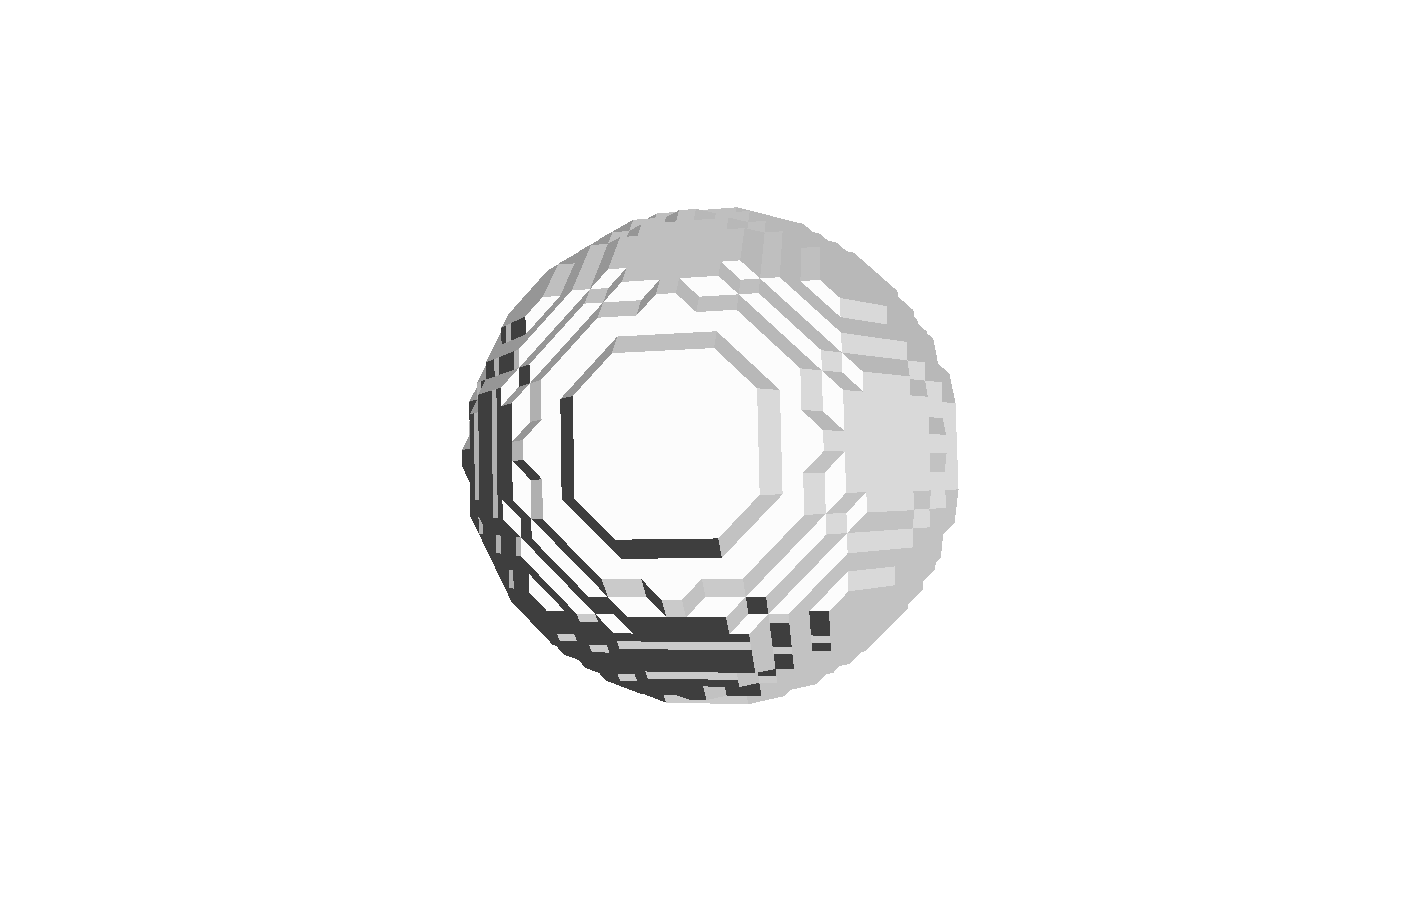
\includegraphics[scale=0.3]{implicitMeshes/sphere.png}
\caption{Sphere}
\end{figure}
\begin{figure}[h]
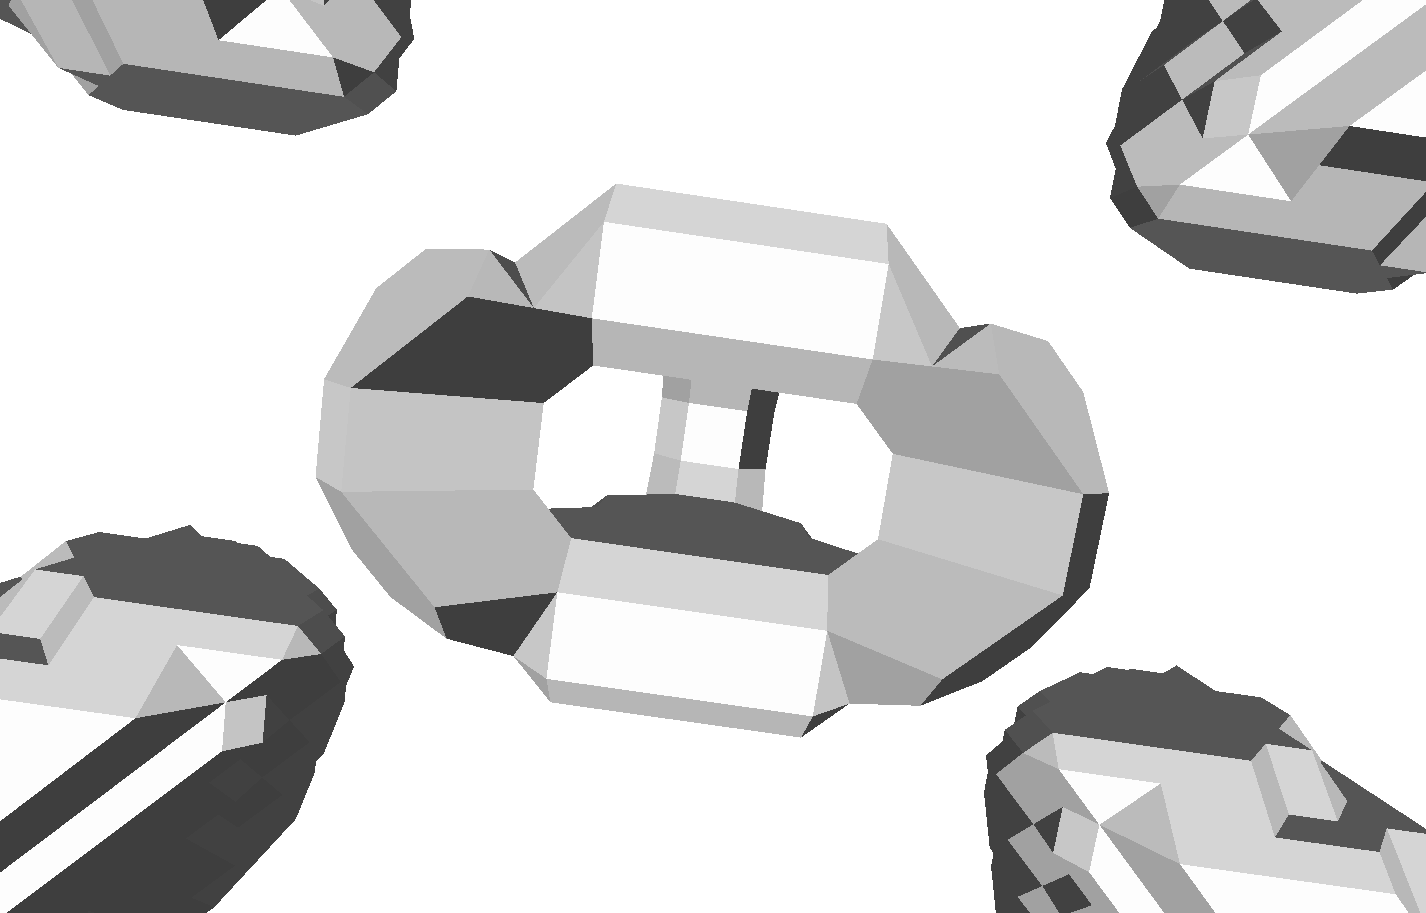
\includegraphics[scale=0.1]{implicitMeshes/genus.png}
\caption{Genus}
\end{figure}

\begin{figure}[h]
    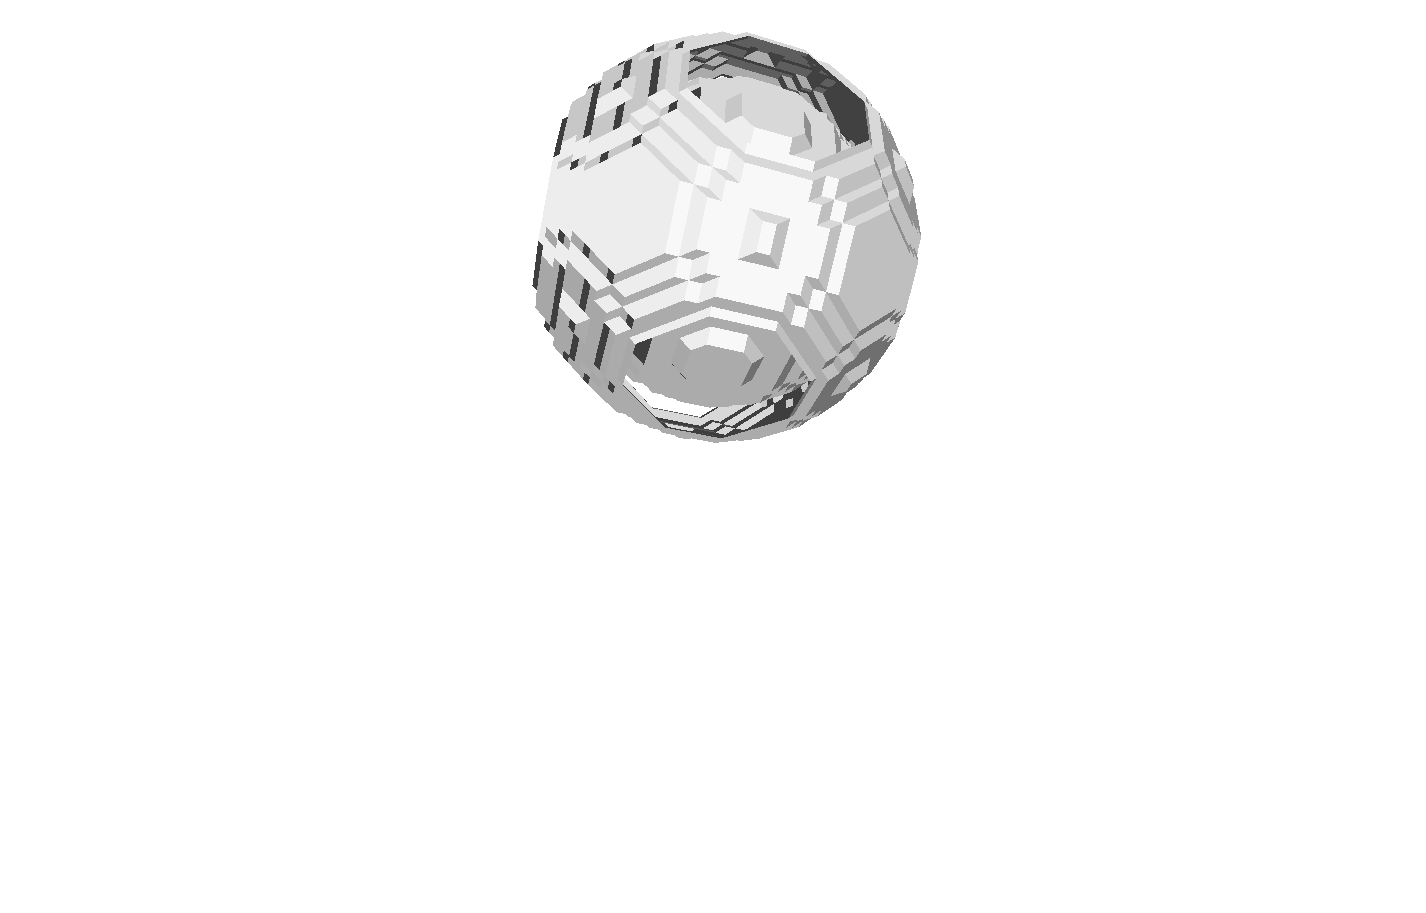
\includegraphics[scale=0.3]{implicitMeshes/sphereWithHole.png}
    \caption{Sphere with hole}
    \end{figure}
    

\begin{figure}[h]
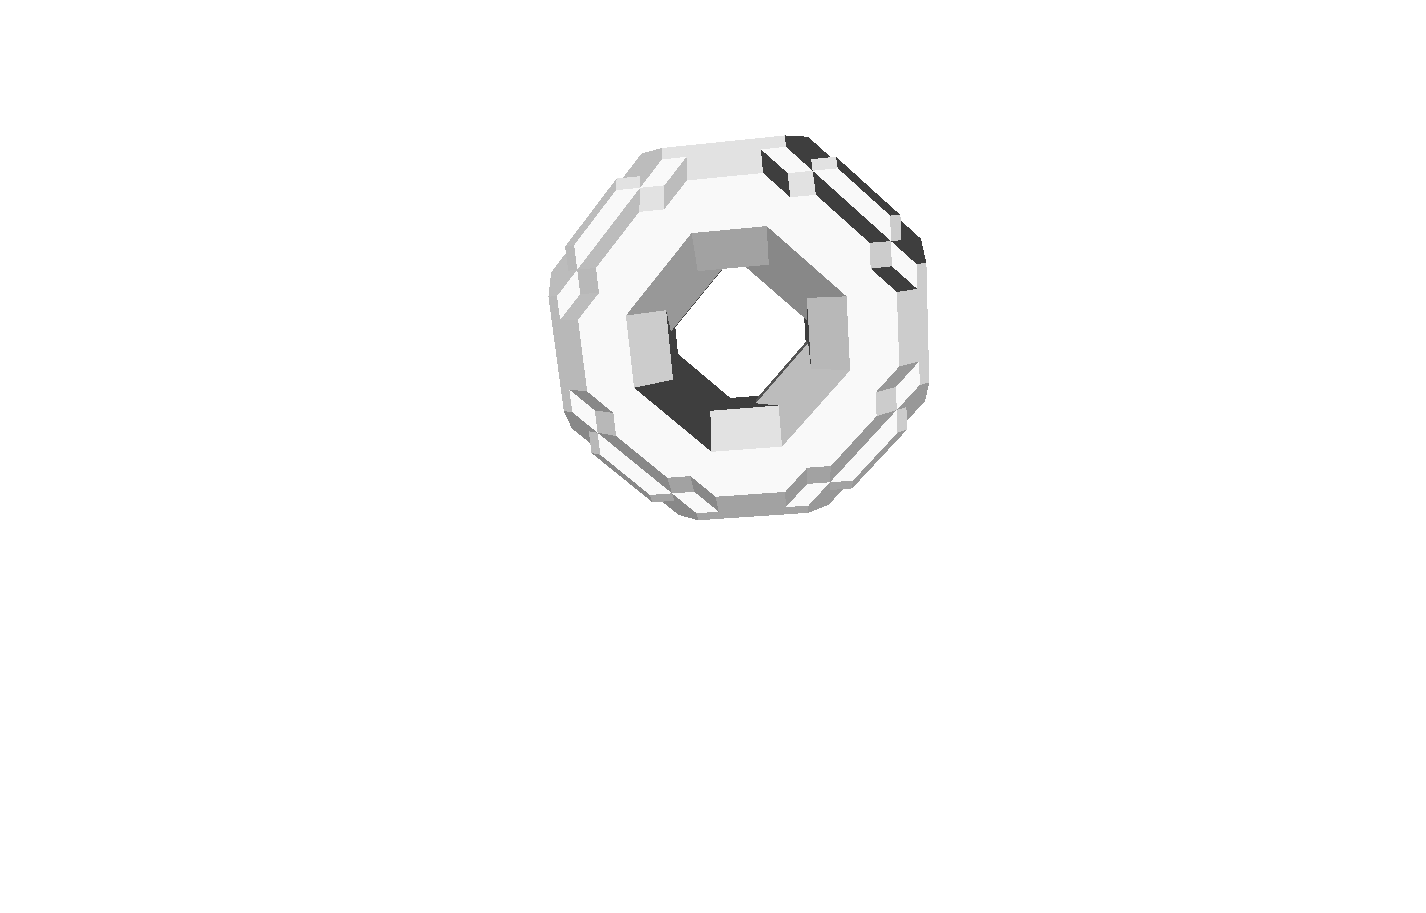
\includegraphics[scale=0.3]{implicitMeshes/torus.png}
\caption{Torus}
\end{figure}

\begin{figure}[h]
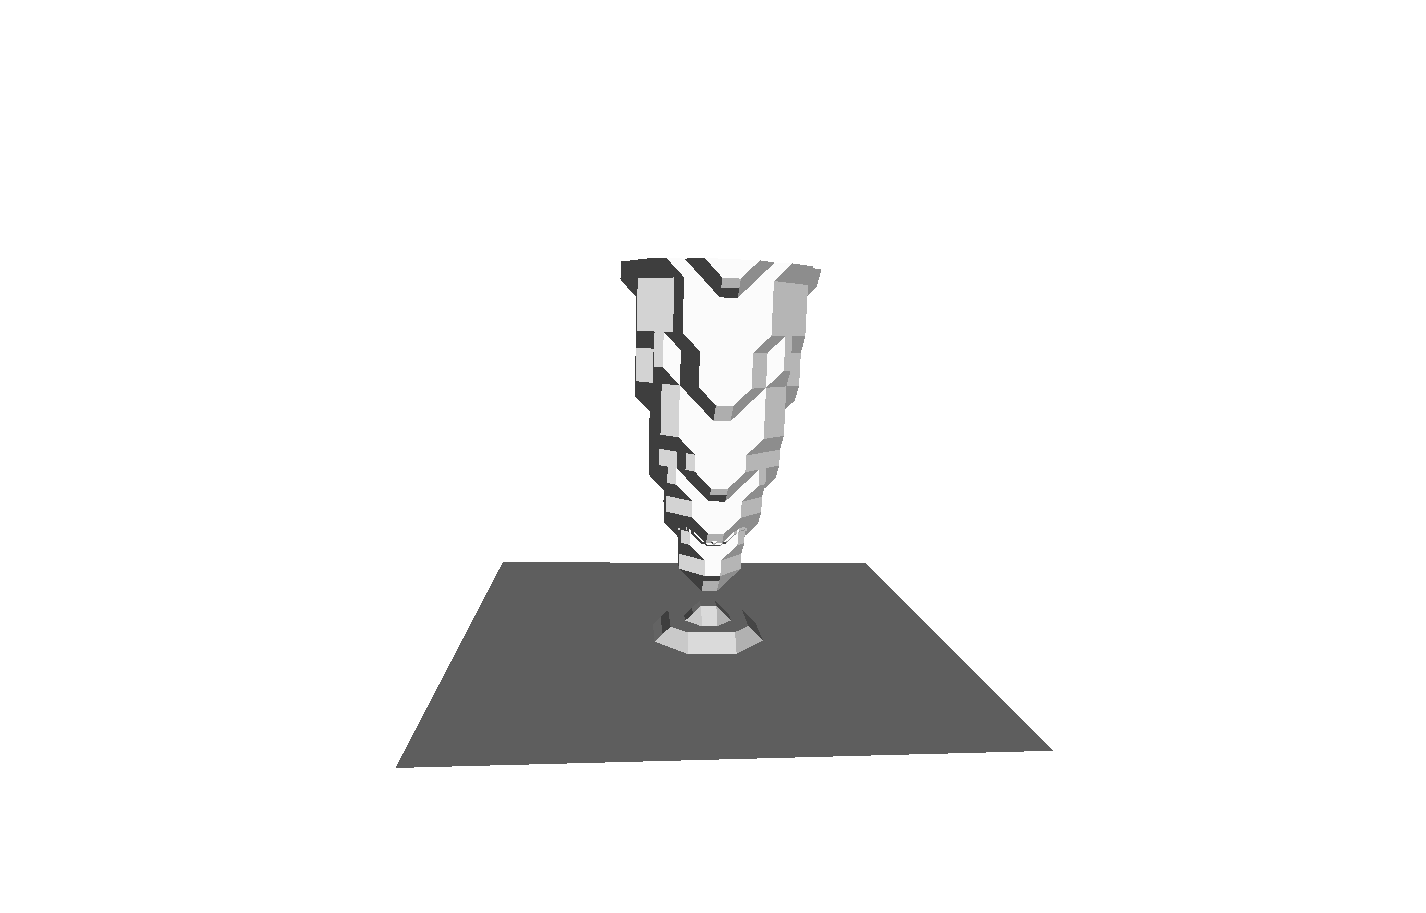
\includegraphics[scale=0.3]{implicitMeshes/wineglass.png}
\caption{Wineglass}
\end{figure}

\clearpage

All of the mesh .off files shown above are contained in the implicitMeshes folder.

Running instructions \\
Optionally switch out which mesh to construct at the bottom half of main function. Default: sphere
1) Evaluate the hardcoded function the default grid \\ 
   ./MarchingCubes   \\
2) Evaluate the hardcoded function on a specified grid \\
  ./Marchingcubes [gridPtsFile] \\


The second mode of the program was used to construct meshes from the output of a neural network
trained to take in 3d coordinates and output the probability that a point lies within a mesh within
the category of meshes the network is trained on. Included in this folder are gifs that illustrate the
result of our Computer Vision project on mesh categories of bench, cellphone, and sofa. 

\begin{figure}[h]
    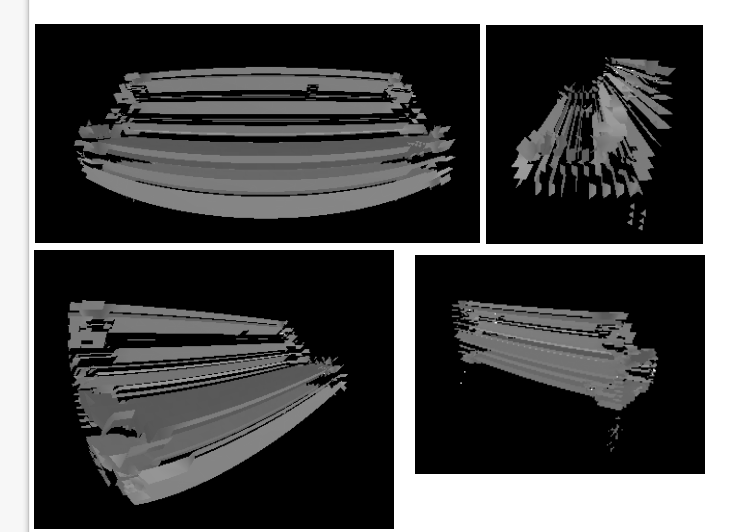
\includegraphics[scale=0.5]{../report/benchImages/benches.png}
    \caption{We trained a network on bench meshes, and this output from the model was conditioned on an input image of a bench from a single orientation}
\end{figure}


Running instructions for this functionality: \\
1) Use provided points and probabilities that point lies on mesh   \\
  ./MarchingCubes [gridPtsFile] [predsFile] \\
2) Same as 3 but outfile will be mesh{x}.off (for scripts generating multiple meshes) \\
  ./MarchingCubes [gridPtsFile] [predsFile] [idForOutFile] \\



\end{document}